% ============================================================
\clearpage
\section{Day 4}
% ============================================================

\subsection{Readings}

\begin{itemize}
    \item iBiology videos.
    \item Erwin Schrödinger, \textit{What Is Life? The Physical Aspect of the Living Cell}.
    \item James D. Watson and Andrew Berry, \textit{DNA: The Secret of Life}.
\end{itemize}


% ============================================================
\subsection{The sameness of things}
% ============================================================

The same physical ideas appear repeatedly across very different biological systems.
Random walks, for example, arise in processes ranging from molecular hopping to the conformations of polymers.
Likewise, similar ideas about binding, switching, cooperativity, and feedback appear in many important regulatory systems.

Examples discussed in the course include:

\begin{enumerate}
    \item \textbf{Chemotaxis}
    \begin{itemize}
        \item V. Sourjik and H. C. Berg, \textit{Receptor sensitivity in bacterial chemotaxis}, PNAS (2002).
        \item J. E. Keymer, R. G. Endres, M. Skoge, Y. Meir, and N. S. Wingreen, \textit{Chemosensing in Escherichia coli: two regimes of two-state receptors}, PNAS (2006).
    \end{itemize}

    \item \textbf{Quorum sensing}
    \begin{itemize}
        \item L. R. Swem, D. L. Swem, N. S. Wingreen, and B. L. Bassler, \textit{Deducing receptor signaling parameters from in vivo analysis: LuxN/AI-1 quorum sensing in Vibrio harveyi}, Cell (2008).
    \end{itemize}

    \item \textbf{Gene expression}
\end{enumerate}


% ============================================================
\subsection{What is life?}
% ============================================================

A useful thought experiment is to ask which properties of life on Earth might be universal and which might simply be particular implementations that arose on Earth.
If life existed elsewhere, some of its organizing principles might be recognizable even if its molecular details were completely different.

\begin{table}[h!]
\centering
\renewcommand{\arraystretch}{1.4}
\begin{tabularx}{0.9\textwidth}{
    |>{\raggedright\arraybackslash}X
    |>{\raggedright\arraybackslash}X|
}
\hline
\textbf{Potentially general feature} & \textbf{Earth-specific implementation that need not be universal}
\\
\hline
A self-replicating blueprint & DNA and its particular molecular structure
\\
\hline
Organization into self-replicating units & Cells as we know them
\\
\hline
Metabolism and energy transduction & Glycolysis, ATP, and particular terrestrial metabolic pathways
\\
\hline
Adaptation and/or evolution & Particular terrestrial evolutionary mechanisms and molecular machinery
\\
\hline
Birth and death of individual systems & Particular cellular life cycles
\\
\hline
A chemical basis for structure and function & CHNOPS chemistry
\\
\hline
Error correction and maintenance of information & Particular DNA-repair and proofreading mechanisms
\\
\hline
\end{tabularx}
\caption{A thought experiment about which features of terrestrial life might reflect general principles of living systems and which may be contingent molecular implementations.}
\end{table}


% ============================================================
\subsubsection{What are the secrets of life?}
% ============================================================

Jacques Monod is reported to have said, ``I think I have discovered the second secret of life.''
Before revealing what he meant, possible candidates for the ``secrets of life'' include:

\begin{itemize}
    \item the structure of DNA and genetic information;
    \item evolution;
    \item enzymes;
    \item genes and inheritance;
    \item self-organization;
    \item cell theory.
\end{itemize}

Monod's ``second secret of life'' was \emph{allostery}.
In the framing used in the lecture, the first secret is the molecular basis of genetic information associated with DNA.


% ============================================================
\subsubsection{Defiance as a characteristic of life}
% ============================================================

One way to think about living systems is through their ability to continually maintain states that would not persist at equilibrium.
Living systems use energy and molecular machinery to ``defy'' passive relaxation toward equilibrium.

Examples include:

\begin{itemize}
    \item creating and maintaining concentration gradients;
    \item performing high-fidelity polymerization despite molecular noise;
    \item adapting to changes in the environment;
    \item enforcing ordered kinetic sequences, or ``socks before shoes'' kinetics;
    \item constructing and maintaining self-organized dissipative structures.
\end{itemize}

The important idea is not that living systems violate thermodynamics.
Rather, they remain out of equilibrium by continually consuming free energy.


% ============================================================
\subsection{Binding by counting}
% ============================================================

Ligand binding can be derived by explicitly counting the microscopic states available to bound and unbound molecules.
This provides a statistical-mechanical route to the same kind of receptor-occupancy formulas encountered earlier using mass-action kinetics.

We use the following notation:

\begin{itemize}
    \item $\Omega$: number of available positions for an unbound ligand;
    \item $L$: number of ligand molecules;
    \item $\epsilon_b<0$: energy of a ligand in the bound state relative to the chosen reference state;
    \item $k_B$: Boltzmann constant;
    \item $T$: absolute temperature;
    \item $\beta=1/(k_BT)$;
    \item $W(L)$: number of ways of arranging $L$ indistinguishable ligands among $\Omega$ available solution positions.
\end{itemize}

For the lattice model,

\begin{equation}
    W(L)=\binom{\Omega}{L}.
\end{equation}


% ------------------------------------------------------------
\subsubsection{From a volume to a lattice model}
% ------------------------------------------------------------

Consider a volume containing ligand molecules and receptors.

\begin{figure}[h!]
\centering
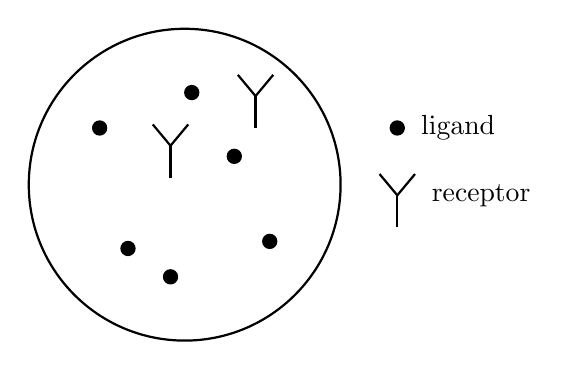
\begin{tikzpicture}[scale=0.9]

    % Volume
    \draw[thick] (0,0) circle (2.2);

    % Ligands
    \foreach \x/\y in {-1.2/0.8,-0.8/-0.9,0.1/1.3,0.7/0.4,1.2/-0.8,-0.2/-1.3} {
        \draw[fill=black] (\x,\y) circle (0.10);
    }

    % Receptor 1
    \draw[thick] (-0.2,0.1) -- (-0.2,0.55);
    \draw[thick] (-0.2,0.55) -- (-0.45,0.85);
    \draw[thick] (-0.2,0.55) -- (0.05,0.85);

    % Receptor 2
    \draw[thick] (1.0,0.8) -- (1.0,1.25);
    \draw[thick] (1.0,1.25) -- (0.75,1.55);
    \draw[thick] (1.0,1.25) -- (1.25,1.55);

    % Labels
    \draw[fill=black] (3.0,0.8) circle (0.10);
    \node[right] at (3.2,0.8) {ligand};

    \draw[thick] (3.0,-0.6) -- (3.0,-0.15);
    \draw[thick] (3.0,-0.15) -- (2.75,0.15);
    \draw[thick] (3.0,-0.15) -- (3.25,0.15);
    \node[right] at (3.35,-0.15) {receptor};

\end{tikzpicture}
\caption{A schematic volume containing ligands and receptors.}
\end{figure}

The continuous three-dimensional volume can be coarse-grained into a lattice of small volume elements.
For counting states, the same idea can be represented even more simply as a one-dimensional array of $\Omega$ boxes.

\begin{figure}[h!]
\centering
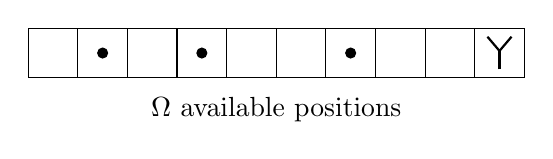
\begin{tikzpicture}[scale=0.9]

    \foreach \i in {0,...,9} {
        \draw (\i*0.7,0) rectangle ++(0.7,0.7);
    }

    % Ligands
    \draw[fill=black] (1.05,0.35) circle (0.07);
    \draw[fill=black] (2.45,0.35) circle (0.07);
    \draw[fill=black] (4.55,0.35) circle (0.07);

    % Receptor
    \draw[thick] (6.65,0.12) -- (6.65,0.38);
    \draw[thick] (6.65,0.38) -- (6.48,0.58);
    \draw[thick] (6.65,0.38) -- (6.82,0.58);

    \node at (3.5,-0.45) {$\Omega$ available positions};

\end{tikzpicture}
\caption{A simplified lattice representation of ligands and a receptor.}
\end{figure}


% ------------------------------------------------------------
\subsubsection*{i) Two boxes and one ligand}
% ------------------------------------------------------------

First consider the simplest possible system.
There is one ligand and one receptor, and the ligand can either remain unbound or occupy the receptor-binding state.

Choose the energy of the unbound state as the reference,

\begin{equation}
    \epsilon_{\mathrm{unbound}}=0.
\end{equation}

The bound state has energy

\begin{equation}
    \epsilon_{\mathrm{bound}}=\epsilon_b,
\end{equation}

with $\epsilon_b<0$ for energetically favorable binding.

The Boltzmann weights of the two states are therefore

\begin{equation}
    w_{\mathrm{unbound}}=1,
\end{equation}

and

\begin{equation}
    w_{\mathrm{bound}}=e^{-\beta\epsilon_b}.
\end{equation}

The partition function is

\begin{equation}
    Z=1+e^{-\beta\epsilon_b}.
\end{equation}

The probability of being bound is therefore

\begin{equation}
    p_b=\frac{e^{-\beta\epsilon_b}}{1+e^{-\beta\epsilon_b}}.
\end{equation}

Equivalently,

\begin{equation}
    \frac{p_b}{1-p_b}=e^{-\beta\epsilon_b}.
\end{equation}


% ------------------------------------------------------------
\subsubsection*{ii) Many boxes and one ligand}
% ------------------------------------------------------------

Now suppose that an unbound ligand can occupy any of $\Omega$ equivalent solution positions.
There are therefore $\Omega$ distinct unbound microstates with energy zero, but only one bound state with energy $\epsilon_b$.

The total statistical weight of the unbound state is

\begin{equation}
    W_{\mathrm{unbound}}=\Omega.
\end{equation}

The statistical weight of the bound state is

\begin{equation}
    W_{\mathrm{bound}}=e^{-\beta\epsilon_b}.
\end{equation}

The partition function is

\begin{equation}
    Z=\Omega+e^{-\beta\epsilon_b}.
\end{equation}

Therefore,

\begin{equation}
    p_b=\frac{e^{-\beta\epsilon_b}}{\Omega+e^{-\beta\epsilon_b}}.
\end{equation}

This can be rewritten as

\begin{equation}
    p_b=\frac{1}{1+\Omega e^{\beta\epsilon_b}}.
\end{equation}

Since

\begin{equation}
    \Omega=e^{\ln\Omega},
\end{equation}

we can write

\begin{equation}
    p_b=\frac{1}{1+\exp\left[\beta\left(\epsilon_b+k_BT\ln\Omega\right)\right]}.
\end{equation}

The quantity

\begin{equation}
    \Delta F=\epsilon_b+k_BT\ln\Omega
\end{equation}

can be interpreted as the free-energy difference between the bound and unbound macrostates.

The energetic contribution $\epsilon_b<0$ favors binding.
The term $k_BT\ln\Omega>0$ represents the entropic cost of restricting a ligand that could otherwise occupy many different positions to a single bound state.
Binding therefore reflects a competition between energy and entropy.


% ------------------------------------------------------------
\subsubsection*{iii) Many boxes and many ligands}
% ------------------------------------------------------------

Now consider $L$ indistinguishable ligands and one receptor.

If the receptor is unbound, all $L$ ligands occupy solution positions.
The number of corresponding microstates is

\begin{equation}
    W(L)=\binom{\Omega}{L}.
\end{equation}

If the receptor is bound, one ligand occupies the receptor and the remaining $L-1$ ligands occupy solution positions.
The number of corresponding solution microstates is therefore

\begin{equation}
    W(L-1)=\binom{\Omega}{L-1}.
\end{equation}

The statistical weight of the unbound macrostate is

\begin{equation}
    W_{\mathrm{unbound}}=W(L).
\end{equation}

The statistical weight of the bound macrostate is

\begin{equation}
    W_{\mathrm{bound}}=W(L-1)e^{-\beta\epsilon_b}.
\end{equation}

Therefore,

\begin{equation}
    p_b=\frac{W(L-1)e^{-\beta\epsilon_b}}{W(L)+W(L-1)e^{-\beta\epsilon_b}}.
\end{equation}

The ratio of multiplicities is

\begin{equation}
    \frac{W(L-1)}{W(L)}=\frac{L}{\Omega-L+1}.
\end{equation}

For a dilute system in which $L\ll\Omega$,

\begin{equation}
    \frac{W(L-1)}{W(L)}\approx\frac{L}{\Omega}.
\end{equation}

Hence

\begin{equation}
    p_b\approx\frac{\frac{L}{\Omega}e^{-\beta\epsilon_b}}{1+\frac{L}{\Omega}e^{-\beta\epsilon_b}}.
\end{equation}

The ratio $L/\Omega$ plays the role of ligand concentration in the lattice model.
Thus increasing ligand concentration increases receptor occupancy.

This statistical-mechanical derivation produces the same general saturating form that appeared earlier in the mass-action treatment of ligand--receptor binding.


% ------------------------------------------------------------
\subsubsection*{Homework: active and inactive receptors}
% ------------------------------------------------------------

Extend the binding-by-counting argument to a receptor that can exist in both an active and an inactive state.
The receptor state introduces additional microstates and energetic contributions that must be included in the statistical weights.


% ============================================================
\subsection{Two receptors and interactions}
% ============================================================

The counting framework can also include interactions between receptors or binding sites.

Consider two receptors and $L$ ligands.
Let $\epsilon_{\mathrm{sol}}$ denote the energy of an unbound ligand in solution, $\epsilon_b$ the binding energy of one ligand, and $\epsilon_{\mathrm{int}}$ an interaction energy that appears when both receptors are occupied.

\begin{table}[h!]
\centering
\renewcommand{\arraystretch}{1.5}
\begin{tabularx}{\textwidth}{
    |>{\centering\arraybackslash}p{2.5cm}
    |>{\raggedright\arraybackslash}X
    |>{\centering\arraybackslash}p{2.5cm}
    |>{\raggedright\arraybackslash}X|
}
\hline
\textbf{State} & \textbf{Energy} & \textbf{Multiplicity} & \textbf{Statistical weight}
\\
\hline
$Y \qquad Y$ &
$L\epsilon_{\mathrm{sol}}$ &
$W(L)$ &
$W(L)e^{-\beta L\epsilon_{\mathrm{sol}}}$
\\
\hline
$Y^{\circ} \qquad Y$ &
$(L-1)\epsilon_{\mathrm{sol}}+\epsilon_b$ &
$W(L-1)$ &
$W(L-1)e^{-\beta[(L-1)\epsilon_{\mathrm{sol}}+\epsilon_b]}$
\\
\hline
$Y \qquad Y^{\circ}$ &
$(L-1)\epsilon_{\mathrm{sol}}+\epsilon_b$ &
$W(L-1)$ &
$W(L-1)e^{-\beta[(L-1)\epsilon_{\mathrm{sol}}+\epsilon_b]}$
\\
\hline
$Y^{\circ} \qquad Y^{\circ}$ &
$(L-2)\epsilon_{\mathrm{sol}}+2\epsilon_b+\epsilon_{\mathrm{int}}$ &
$W(L-2)$ &
$W(L-2)e^{-\beta[(L-2)\epsilon_{\mathrm{sol}}+2\epsilon_b+\epsilon_{\mathrm{int}}]}$
\\
\hline
\end{tabularx}
\caption{States, energies, multiplicities, and statistical weights for two interacting receptor-binding sites.}
\end{table}

If the two singly-bound states are grouped together into one macrostate, their total multiplicity is

\begin{equation}
    2W(L-1).
\end{equation}

The interaction energy $\epsilon_{\mathrm{int}}$ represents energetic coupling between the two occupied receptors.
If $\epsilon_{\mathrm{int}}<0$, simultaneous occupancy is energetically favored.
If $\epsilon_{\mathrm{int}}>0$, simultaneous occupancy is energetically penalized.


% ============================================================
\subsection{Bicoid gradients}
% ============================================================

Bicoid is a transcription factor that forms a concentration gradient along the anterior--posterior axis of the early \textit{Drosophila} embryo.
Target genes respond to the local Bicoid concentration through Bicoid binding to regulatory DNA.
This provides a biological example in which a spatial concentration profile can be translated into different binding occupancies and therefore different patterns of gene expression.


% ============================================================
\subsection{Allostery: the second secret of life}
% ============================================================

The word \emph{allostery} comes from the Greek \emph{allos}, meaning ``other'', and \emph{stereos}, meaning ``solid'' or ``structure''.
In an allosteric protein, a regulatory molecule binds at a site that is physically distinct from the protein's active or functional site.
Binding at the regulatory site changes the energetic or conformational state of the protein and thereby alters activity at the other site.

The central idea is therefore coupling between spatially distinct sites on the same molecular system.

Ligand-based feedback of this kind is widespread in biology.
Metabolic pathways provide many examples in which metabolites regulate enzymes upstream or downstream in the pathway.
Glycolysis, which converts glucose into pyruvate, contains several such regulatory steps.

Allostery provides a molecular mechanism through which a protein can sense one chemical signal and alter its response to another.

% ------------------------------------------------------------
\subsubsection{Statistical mechanics of allosteric enzymes}
% ------------------------------------------------------------

A useful framework for describing allosteric enzymes is the Monod-Wyman-Changeux (MWC) model.
In this picture, an enzyme can fluctuate between different conformational states, commonly an active state and an inactive state.
These states can have different substrate-binding affinities and different catalytic activities.
The relative probabilities of the states, together with ligand binding, determine the overall activity of the enzyme.

The same states-and-weights idea used for ligand binding can therefore be extended to allostery.
Instead of considering only bound and unbound states, we enumerate combinations of conformational state and ligand occupancy, assign each state an appropriate statistical weight, and normalize over all possible states.

A useful reference is:

\begin{quote}
T. Einav, L. Mazutis, and R. Phillips,
\textit{Statistical Mechanics of Allosteric Enzymes},
arXiv:1701.03988 (2017).
\end{quote}

The paper first reformulates Michaelis--Menten kinetics using a states-and-weights language and then extends this framework to MWC enzymes, allosteric regulators, competitive inhibitors, and enzymes with multiple substrate-binding sites.